\documentclass{beamer}
\usetheme{Feather}
% \usecolortheme{default}
\usepackage{hyperref}
\definecolor{links}{HTML}{2A1B81}
\definecolor{green}{HTML}{008000}
\hypersetup{colorlinks,linkcolor=,urlcolor=links}
\usepackage[utf8]{inputenc} % this is needed for german umlauts
\usepackage[english]{babel} % this is needed for german umlauts
\usepackage[T1]{fontenc}    % this is needed for correct output of umlauts in pdf
\usepackage{pifont}
\usepackage{graphicx}
\usepackage{minted} % needed for the inclusion of source code
\usepackage{csquotes}


\newcommand{\FolderOpen}[1][.8\ht\strutbox]{%
      \includegraphics[height=#1]{graphics/FolderOpen}%
    }

\newcommand{\FileImage}[1][.8\ht\strutbox]{%
      \includegraphics[height=#1]{graphics/file}%
    }

\begin{document}

\title{Software Engineering Basics}
% \subtitle{A subtitle}
\author{Martin Thoma}
\date{14. August 2018}
\subject{Software Engineering}

\frame{\titlepage}

\section{Intended Audience}
\subsection{A subsection!}
\begin{frame}{Intended Audience}
    Software is written by people with different backgrounds and strengths. Not
    everybody has a Software Engineering background. Those slides should help
    you to get the basics.
\end{frame}

\subsection{A subsection!}
\begin{frame}{Alice and Bob}
    \begin{columns}
        \begin{column}{0.5\textwidth}
             
\includegraphics[width=1.0\textwidth]{graphics/car.jpg}
        \end{column}
        \begin{column}{0.5\textwidth}
            \begin{itemize}
                \item Project: Build self-driving car
                \item Alice is in the US, Bob in Germany
            \end{itemize}
        \end{column}
    \end{columns}
\end{frame}

% \subsection{Version Control}
\begin{frame}{Project structure}
    \begin{columns}
        \begin{column}{0.5\textwidth}
            \begin{itemize}
                \item[\FolderOpen] bin
                \item[\FolderOpen] docs
                \item[\FolderOpen] awesome\_project
                \item[\FolderOpen] tests
                \item[\FileImage] setup.py
                \item[\FileImage] tox.ini
            \end{itemize}
        \end{column}
        \begin{column}{0.5\textwidth}
            \begin{itemize}
                \item[\textcolor{green}{\ding{58}}] \texttt{\$ grep -rnIi foobar}
            \end{itemize}
            Details on \href{https://martin-thoma.com/python-projects/}{my blog}.
        \end{column}
    \end{columns}
\end{frame}

\begin{frame}{git workflow}
    \begin{enumerate}
        \item \texttt{\$ git clone repostory.git}
        \item \texttt{\$ git add filename}
        \item \texttt{\$ git commit}
        \item \texttt{\$ git push}
    \end{enumerate}

    \uncover<2>{\includegraphics[width=1.0\textwidth,height=0.5\textheight,keepaspectratio]{graphics/git-workflow.png}}
\end{frame}

\begin{frame}{Version Control: git}
    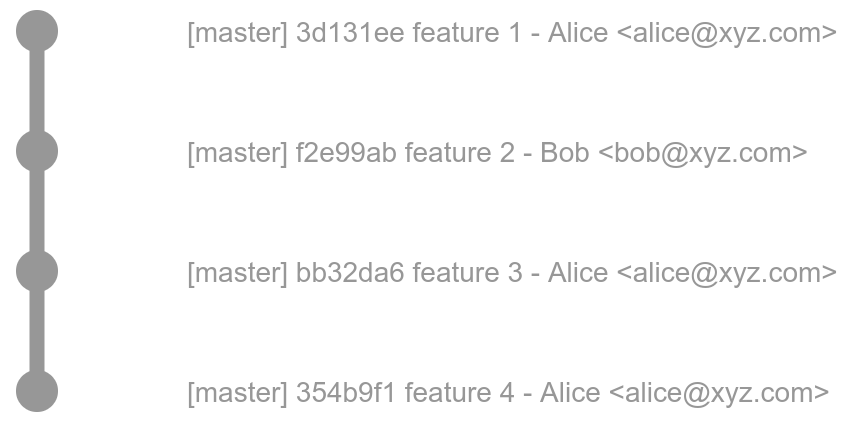
\includegraphics[width=1.0\textwidth]{graphics/git-simple.png}
\end{frame}

\begin{frame}{git log}
    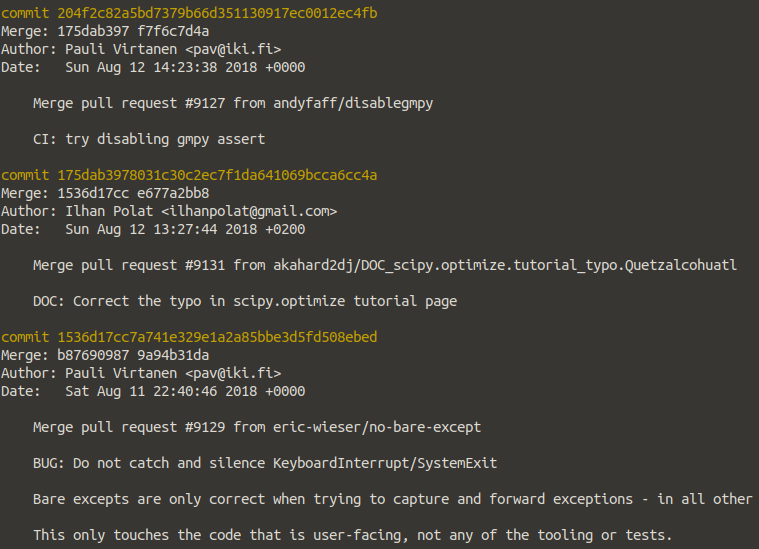
\includegraphics[width=0.9\textwidth]{graphics/git-log.png}
\end{frame}

\begin{frame}{git blame}
    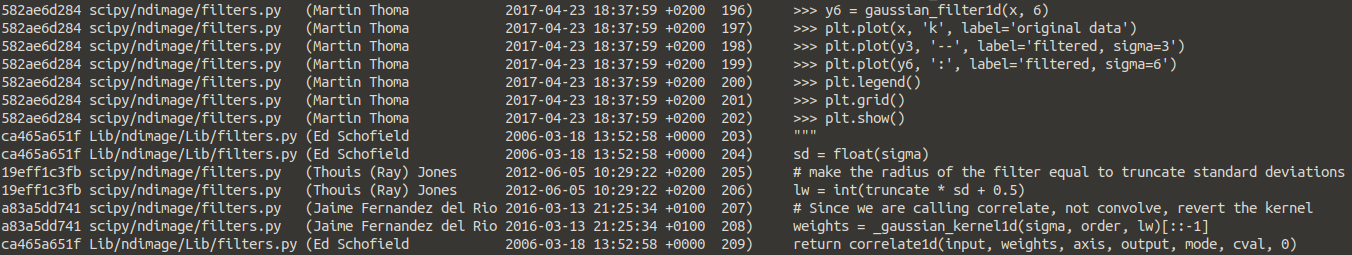
\includegraphics[width=1.0\textwidth]{graphics/git-blame.png}
\end{frame}

\begin{frame}{git status}
    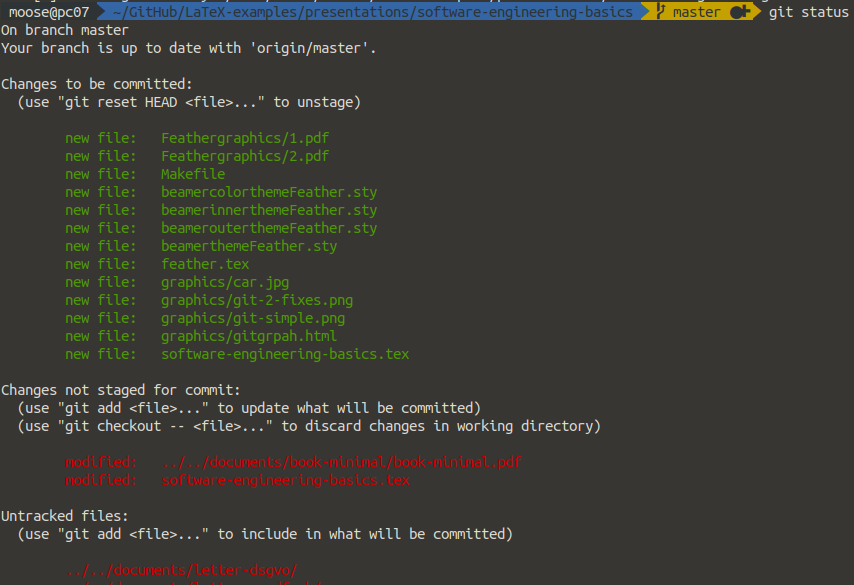
\includegraphics[width=1.0\textwidth]{graphics/git-status.png}
\end{frame}

\begin{frame}{}
     \huge We read code MUCH more often than we write it.
\end{frame}

\begin{frame}{git}
    Problem: Dirty commit history due to bugs / fixes
    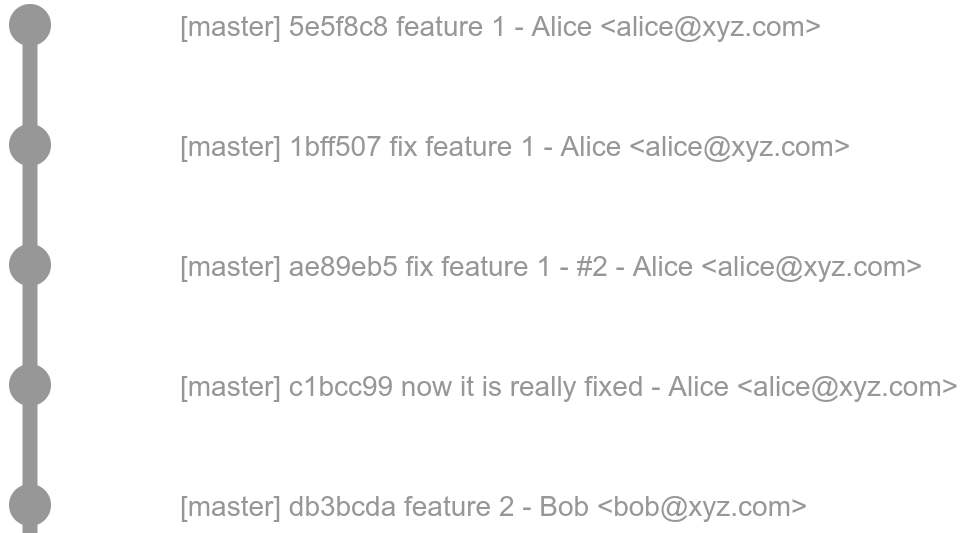
\includegraphics[width=1.0\textwidth]{graphics/git-2-fixes.png}
\end{frame}

\begin{frame}{Auto formatting}
    \begin{itemize}[<+->]
        \item PRs should not be about simple code style
        \item Choose one \href{https://martin-thoma.com/python-style-guide/}{style guide}
              and stick to it
        \item Trailing spaces are just noise - make your editor remove them
              automatically.
    \end{itemize}
\end{frame}

\begin{frame}{The Zen of Python, by Tim Peters (1)}
Beautiful is better than ugly.\\
Explicit is better than implicit.\\
Simple is better than complex.\\
Complex is better than complicated.\\
Flat is better than nested.\\
Sparse is better than dense.\\
Readability counts.\\
Special cases aren't special enough to break the rules.\\
Although practicality beats purity.\\
Errors should never pass silently.\\
Unless explicitly silenced.
\end{frame}

\begin{frame}{The Zen of Python, by Tim Peters (2)}
In the face of ambiguity, refuse the temptation to guess.\\
There should be one-- and preferably only one --obvious way to do it.\\
Although that way may not be obvious at first unless you're Dutch.\\
Now is better than never.\\
Although never is often better than *right* now.\\
If the implementation is hard to explain, it's a bad idea.\\
If the implementation is easy to explain, it may be a good idea.\\
Namespaces are one honking great idea -- let's do more of those!
\end{frame}

\begin{frame}{commit squashing}
    \begin{columns}
        \begin{column}{0.5\textwidth}
            \textbf{Commit squashing}

            Making multiple commits in a row become one
        \end{column}
        \begin{column}{0.5\textwidth}
            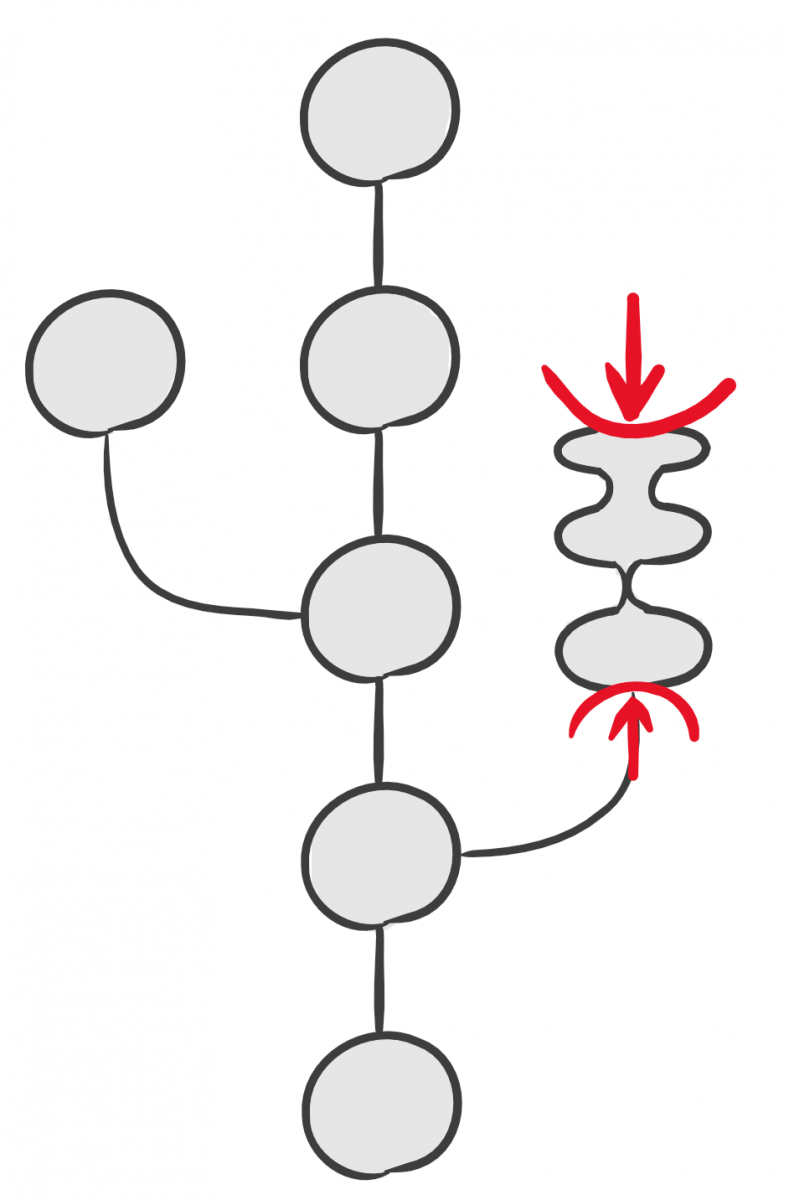
\includegraphics[height=0.5\textheight]{graphics/commit-squashing.png}
            {\small Image source: \href{https://stevenschwenke.de/GitToSquashOrNotToSquash}{stevenschwenke.de}}
        \end{column}
    \end{columns}
\end{frame}

\begin{frame}{git merge}
    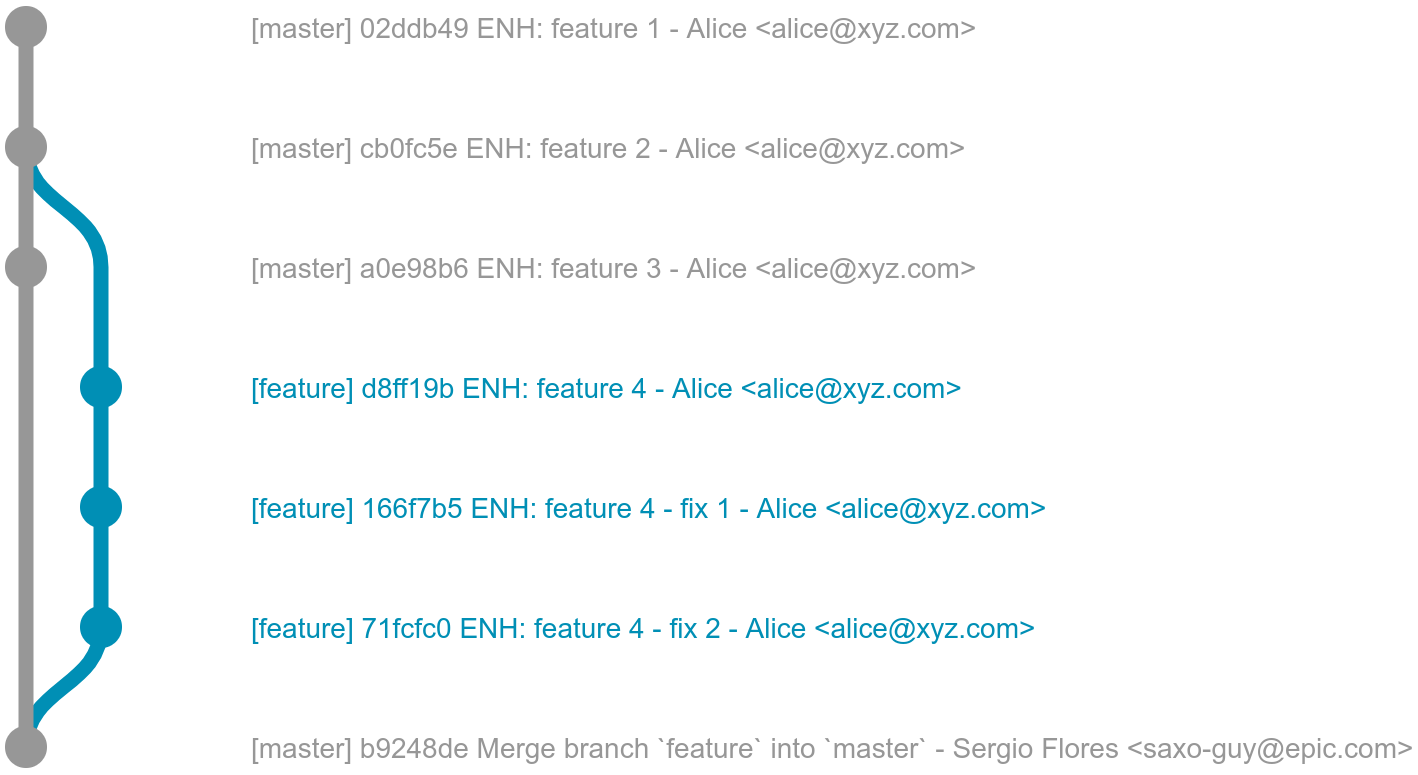
\includegraphics[width=1.0\textwidth,height=0.5\textheight,keepaspectratio]{graphics/git-merge.png}
\end{frame}

\begin{frame}{git merge vs git rebase}
    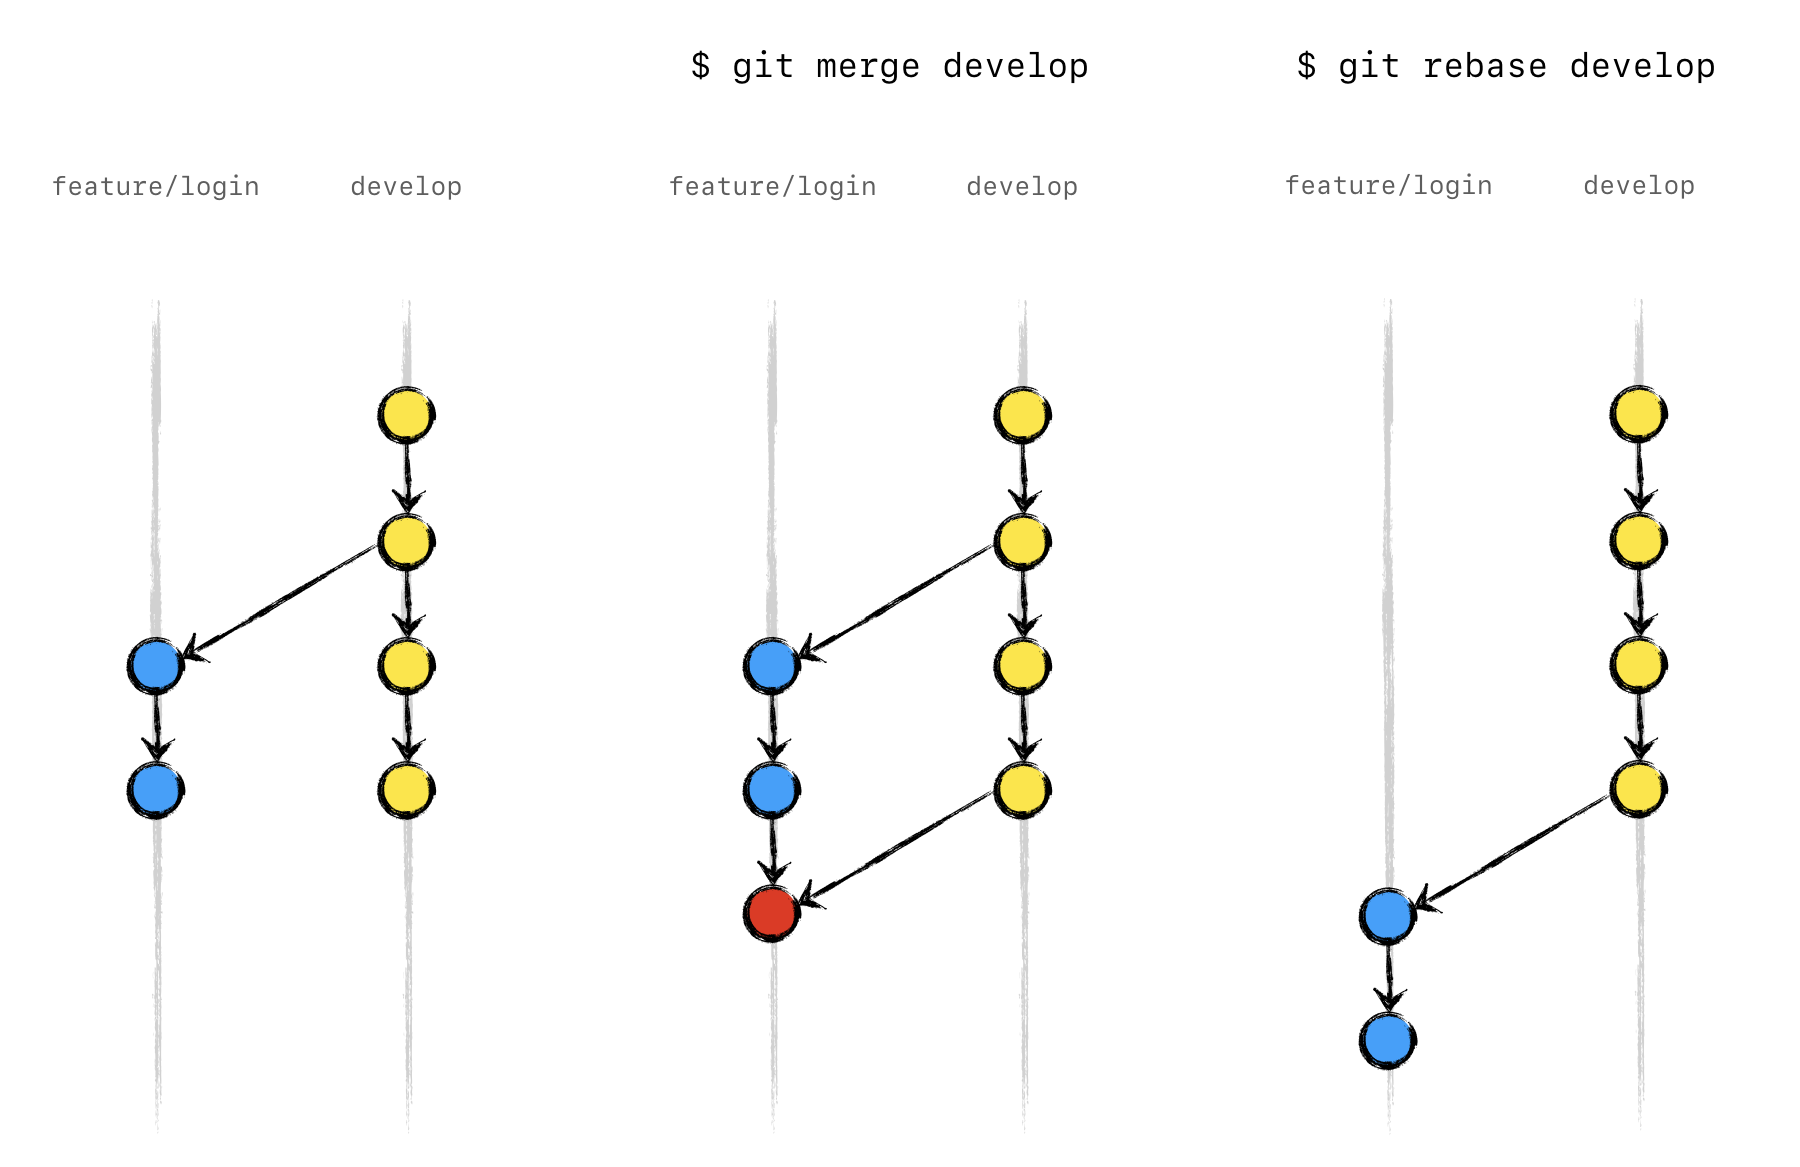
\includegraphics[width=1.0\textwidth,height=0.8\textheight,keepaspectratio]{graphics/git-rebase.png}

    {\small Image source: \href{https://jeffkreeftmeijer.com/git-rebase/}{Jeff Kreeftmeijer}}
\end{frame}


\section{Bugs}
\begin{frame}{Logic Bugs: Functions and McCabe}
\inputminted[linenos,
             numbersep=7pt,
             fontsize=\footnotesize, tabsize=4]{python}{src/sieve-v1.py}
\end{frame}

\begin{frame}{Logic Bugs: Names}
\inputminted[linenos,
             numbersep=7pt,
             fontsize=\footnotesize, tabsize=4,
             firstline=4]{python}{src/sieve-v2.py}
\end{frame}

\begin{frame}{Logic Bugs: Doctests!}
\inputminted[linenos,
               numbersep=7pt,
                fontsize=\footnotesize, tabsize=4,
                firstline=8, lastline=24]{python}{src/sieve-v3.py}
\end{frame}


\section{Falsehood Data Scientists Beliefes}
\begin{frame}{Falsehood Data Scientists Beliefes}
\begin{centering}
(1) Floating point numbers always look like this: 1.23456 or 0.000004577 or 12345.467765.
\end{centering}

\uncover<2->{
    \begin{itemize}
        \item<2-> Scientific notation: \texttt{4.577E-5} or \texttt{1.2345467765E4}
        \item<3-> German decimal format: \texttt{1,23456} or \texttt{0,000004577}
    \end{itemize}
}
\end{frame}

\begin{frame}{Falsehood Data Scientists Beliefes}
\begin{centering}
(2.1) Country names have an unique representation
\end{centering}

\uncover<2>{
    \enquote{Germany} vs \enquote{Deutschland}
}
\end{frame}

\begin{frame}{Falsehood Data Scientists Beliefes}
\begin{centering}
(2.2) Country names have an unique representation in English
\end{centering}

\uncover<2>{
     \enquote{United Kingdom} vs \enquote{UK}
}
\end{frame}

\begin{frame}{Falsehood Data Scientists Beliefes}
\begin{centering}
(2.3) Country names have an unique unabreviated representation in English
\end{centering}

\uncover<2>{
    \enquote{United Kingdom} vs \enquote{Great Britain} vs \enquote{England}
}
\uncover<3>{Solution: Use/Demand \textbf{ISO 3166-1 alpha-3 country codes} everywhere}
\end{frame}

\begin{frame}{Falsehood Data Scientists Beliefes}
\begin{centering}
(3) Data is clean
\end{centering}

\uncover<2->{
    No.
    \begin{itemize}
        \item<3-> User database: Birth date in the year 3.
        \item<4-> User database: Active user who is more than 90 years old.
        \item<5-> User database: User who is younger than 6.
    \end{itemize}
}
\end{frame}

\begin{frame}{Falsehood Data Scientists Beliefes}
\begin{centering}
(4) Time has no beginning and no end
\end{centering}

\uncover<2->{
    Unix Time Stamp: Seconds since 1st of January, 1970. Stored in unsigned int.
}
\end{frame}

\begin{frame}{Falsehood Data Scientists Beliefes}
\begin{centering}
(4) To avoid the Year-2038 problem, I can store \texttt{YYYY-mm-dd HH:MM:ss}
\end{centering}

\uncover<2->{
    \begin{itemize}
        \item<2-> \href{http://strftime.org/}{Python's strftime directives}
        \item<3-> Timezones
        \item<4-> Whenever possible, store the timezone and use \textbf{ISO 8601}:
                  \texttt{2012-04-23T18:25:43.511+02:30} (\href{https://stackoverflow.com/a/15952652/562769}{reasons})
    \end{itemize}
}
\end{frame}


\begin{frame}{Falsehood Data Scientists Beliefes}
\begin{centering}
(5) The (physical) unit of a column / an API can be guessed.
\end{centering}

\uncover<2->{
    \begin{itemize}
        \item<2-> Clarify it
        \item<3-> See if the distribution / quantiles are reasonable
        \item<4-> Internally, use unit library \href{http://pint.readthedocs.io/en/latest/}{Pint}
    \end{itemize}
}
\end{frame}


\begin{frame}{See also}
    \begin{itemize}
        \item git
        \begin{itemize}
            \item \href{http://meldmerge.org/}{meld}: Tool for diff and merge (\texttt{\$ git mergetool})
            \item \href{https://nvie.com/posts/a-successful-git-branching-model/}{A successful Git branching model}
        \end{itemize}
        \item \href{https://www.youtube.com/watch?v=8SNaW1nt6j0}{Debugging Python with ipdb and Sypder} - starting at 4:00
        \item \href{https://docs.python.org/3/library/profile.html}{cprofile}: Check where code improvements are effective
        \item David Goldberg: \href{https://www.itu.dk/~sestoft/bachelor/IEEE754_article.pdf}{What Every Computer Scientist Should Know About Floating-Point Arithmetic}
        \item \href{https://martin-thoma.com/testing-python-code/}{Testing with Python}
        \item \href{https://martin-thoma.com/logging-in-python/}{Logging with Python}
        \item UML: \href{https://www.websequencediagrams.com/}{Sequence diagrams}, Flow charts (e.g. \href{https://wiki.gnome.org/Apps/Dia/}{Dia} or \href{https://www.draw.io/}{draw.io})
        \item \href{https://balsamiq.com/}{Balsamiq}: Draft an UI
        \item Web: \href{https://gist.github.com/alexserver/2fcc26f7e1ebcfc9f6d8}{REST basics}
    \end{itemize}
\end{frame}
\end{document}
Bare excepts are only correct when trying to capture and forward exceptions - in all other cases, except Exception should be used to avoid catching KeyboardInterrupt.